% Exportación completa del documento de Google Drive.
% Requiere en el preámbulo: \usepackage{graphicx}, \usepackage{tabularx} y \usepackage{booktabs}.
% Las figuras extraídas se encuentran en la carpeta figuras_drive/.

\chapter{Diseño del sistema de control}

Este capítulo presenta el diseño del sistema desarrollado para controlar un dron Crazyflie 2.1 mediante diferentes interfaces. Primero se describen la arquitectura de comunicación y las medidas de seguridad establecidas para las pruebas de vuelo. Posteriormente, se presentan las interfaces preliminares de control mediante botones, gestos de mano y un marcador del ecosistema Robotat. Estas etapas permitieron validar progresivamente la comunicación, la generación de referencias de movimiento y la supervisión del vuelo antes de integrar el sistema de reconocimiento de gestos corporales.

Para implementar el sistema se utilizó Python 3.11.9 junto con la biblioteca oficial cflib de Bitcraze. Esta biblioteca permitió establecer la comunicación con el dron, recibir su telemetría y enviar referencias de posición y velocidad. También se utilizaron las herramientas oficiales de Bitcraze para actualizar el firmware y verificar el identificador uniforme de recursos (URI, por sus siglas en inglés de Uniform Resource Identifier) correspondiente al Crazyflie.

Antes de integrar las interfaces de control se realizaron vuelos preliminares para comprobar el estado de los motores, la comunicación por radio y la estabilidad básica del dron. Estas pruebas permitieron identificar las condiciones mínimas de seguridad necesarias para continuar con el desarrollo.

\section{Medidas de seguridad}

Antes de implementar movimientos complejos, se definieron las condiciones de seguridad que debía cumplir el sistema. El objetivo de esta etapa fue reducir la posibilidad de pérdida de control, impedir que el dron abandonara el espacio de captura confiable y detectar fallas en la estimación de posición antes de que representaran un riesgo para el usuario o para el equipo.

Durante las primeras pruebas se observaron desviaciones respecto del vuelo estacionario, pérdidas temporales de información procedente de Robotat y diferencias entre la posición medida externamente y la posición estimada por el Crazyflie. Por esta razón, se establecieron mecanismos de protección antes de incorporar el reconocimiento de gestos.

\subsection{Delimitación del área de vuelo}

El ecosistema Robotat dispone de un volumen aproximado de $4\times 5\times 2\ m$. Dentro de este espacio se definió un volumen de operación de $2\times 2\times 1.5\ m$, destinado específicamente a las pruebas de vuelo desarrolladas en este trabajo. La Figura~\ref{fig:drive_01} presenta la relación entre el volumen disponible y el área seleccionada.

\begin{figure}[htbp]
    \centering
    \caption{Área de trabajo definida dentro del ecosistema Robotat.}
    \label{fig:drive_01}
    \IfFileExists{figuras/area_trabajo_robobtat.pdf}{%
        \includegraphics[width=0.72\textwidth]{figuras/area_trabajo_robobtat.pdf}%
    }{%
        \fbox{\parbox[c][4cm][c]{0.72\textwidth}{\centering Imagen pendiente: \texttt{figuras/area\_trabajo\_robobtat.pdf}}}%
    }

    \begin{minipage}{0.72\textwidth}
        \footnotesize
        \textit{Nota.} La figura representa el volumen total disponible en el ecosistema Robotat y el área definida para la operación del cuadricóptero. Elaboración propia.
    \end{minipage}
\end{figure}

La delimitación permitió restringir los movimientos a una región en la que la detección de los marcadores presentaba un comportamiento confiable. También permitió establecer límites conocidos para las referencias de posición generadas por las interfaces de control.

\subsection{Procedimiento de prevuelo}

Antes del despegue se verificaban la comunicación con el Crazyflie y la disponibilidad de una medición de Robotat con una antigüedad no mayor de 0.75 s. En el controlador preliminar, las posiciones externas se enviaban al dron aproximadamente a 20 Hz; en la versión definitiva se transmitía cada cuadro distinto recibido desde Robotat.

También se comprobaba la convergencia del filtro de Kalman extendido (EKF), comparando la posición estimada por el dron con la medida por Robotat. Para autorizar el despegue, la distancia entre ambas debía permanecer por debajo de 0.07 m durante al menos 1 s. Si esta condición no se alcanzaba en un máximo de 12 s, o faltaban mediciones recientes, el prevuelo se consideraba fallido y se impedía continuar.

\subsection{Supervisión durante el vuelo}

La comparación entre la posición estimada y la posición externa se mantuvo durante el vuelo. El controlador preliminar utilizó un límite mayor que el aplicado durante el prevuelo, debido a que los movimientos podían producir diferencias transitorias entre ambas estimaciones.

Se consideraba una divergencia cuando la distancia entre ambas posiciones superaba 0.15 m. Al alcanzar esta condición, el supervisor activaba la respuesta de emergencia.

La supervisión se ejecutaba de forma paralela al control del vuelo. El monitor comprobaba periódicamente la disponibilidad de una pose reciente, el error entre el EKF y el sistema de captura de movimiento, y el estado general de la operación. De esta manera, una interrupción en la actualización de posición podía detectarse independientemente de las órdenes emitidas desde la interfaz.

\subsection{Respuesta ante emergencias}

El paro de emergencia podía activarse manualmente o por el supervisor de seguridad. En el controlador preliminar, se activaba automáticamente si Robotat dejaba de proporcionar una pose reciente o si la diferencia entre la posición estimada y la medida superaba 0.15 m. Además, los fallos detectados al enviar órdenes de despegue, movimiento, seguimiento o aterrizaje podían activar este mecanismo.

Al activarse el paro, se interrumpía la trayectoria del comandante de alto nivel y se transmitía repetidamente una orden de detención. Esta respuesta se distinguía del rechazo de una referencia fuera del área permitida: rechazar una orden impedía ejecutarla, mientras que el paro interrumpía la operación y bloqueaba nuevos comandos.

Después de una emergencia, el controlador permanecía en un estado de enclavamiento que impedía aceptar nuevas órdenes de movimiento o despegue. Para reanudar la operación era necesario reiniciar el sistema y ejecutar nuevamente el procedimiento de prevuelo. Esta condición evitaba que el operador reanudara accidentalmente el vuelo sin comprobar la comunicación, la disponibilidad de la pose externa y la convergencia del estimador.

\section{Arquitectura de comunicación}

La operación del sistema se basó en la interacción entre la computadora, el ecosistema Robotat y el firmware del Crazyflie. La cadena principal de control se presenta en la Figura~\ref{fig:drive_02}.

\begin{figure}[htbp]
    \centering
    \caption{Cadena principal de control utilizada para operar el Crazyflie.}
    \label{fig:drive_02}
    \IfFileExists{figuras/cadena_principal_control.pdf}{%
        \includegraphics[width=0.82\textwidth]{figuras/cadena_principal_control.pdf}%
    }{%
        \fbox{\parbox[c][4cm][c]{0.82\textwidth}{\centering Imagen pendiente: \texttt{figuras/cadena\_principal\_control.pdf}}}%
    }

    \begin{minipage}{0.82\textwidth}
        \footnotesize
        \textit{Nota.} La figura muestra el flujo desde la acción del operador hasta la ejecución de las órdenes por los motores del dron. Elaboración propia.
    \end{minipage}
\end{figure}

La computadora recibía las acciones del operador mediante la interfaz correspondiente. Posteriormente, el módulo de seguridad verificaba que la orden cumpliera las restricciones del área de trabajo y que existieran datos válidos de posicionamiento. Una vez validadas estas condiciones, las referencias se enviaban al dron mediante Crazyradio. De forma paralela, Robotat proporcionaba la pose externa del Crazyflie. La computadora recibía esta información mediante el protocolo MQTT (\textit{Message Queuing Telemetry Transport}), validaba las mediciones y las transmitía al estimador del dron. Este flujo de realimentación se presenta en la Figura~\ref{fig:drive_03}.

\begin{figure}[htbp]
    \centering
    \caption{Flujo de realimentación externa para la estimación del estado del Crazyflie.}
    \label{fig:drive_03}
    \IfFileExists{figuras/Flujo_realimentacion_externa.pdf}{%
        \includegraphics[width=0.82\textwidth]{figuras/Flujo_realimentacion_externa.pdf}%
    }{%
        \fbox{\parbox[c][4cm][c]{0.82\textwidth}{\centering Imagen pendiente: \texttt{figuras/Flujo\_realimentacion\_externa.pdf}}}%
    }

    \begin{minipage}{0.82\textwidth}
        \footnotesize
        \textit{Nota.} La figura representa el flujo de datos desde Robotat hasta el filtro de Kalman extendido del Crazyflie. Elaboración propia.
    \end{minipage}
\end{figure}

\section{Interfaz preliminar mediante botones}

Después de establecer las condiciones de seguridad, se desarrolló una interfaz gráfica para realizar pruebas de control individual. La interfaz se implementó en Python mediante Tkinter y reunió en una sola ventana las funciones de conexión, validación previa al vuelo, generación de movimientos, supervisión de telemetría y respuesta ante emergencias.

Esta interfaz facilitó la operación durante las pruebas, ya que las acciones principales podían ejecutarse desde un entorno gráfico. También sirvió como base para integrar posteriormente las interfaces gestuales.

La Figura~\ref{fig:drive_04} presenta la interfaz y sus principales áreas funcionales.

\begin{figure}[htbp]
    \centering
    \caption{Interfaz gráfica para el control individual del Crazyflie.}
    \label{fig:drive_04}
    \IfFileExists{figuras/gui_control_botones.pdf}{%
        \includegraphics[width=0.72\textwidth]{figuras/gui_control_botones.pdf}%
    }{%
        \fbox{\parbox[c][4cm][c]{0.72\textwidth}{\centering Imagen pendiente: \texttt{figuras/gui\_control\_botones.pdf}}}%
    }

    \begin{minipage}{0.72\textwidth}
        \footnotesize
        \textit{Nota.} La figura muestra el encabezado, la configuración del dron, los comandos principales, los controles de movimiento, la telemetría y la función de exportación. Elaboración propia.
    \end{minipage}
\end{figure}

La interfaz se dividió en las siguientes áreas:

\begin{enumerate}
    \item \textbf{Encabezado:} mostraba el nombre de la prueba y una descripción del tipo de control.
    \item \textbf{Configuración del dron:} presentaba la URI de radio y el tópico de Robotat.
    \item \textbf{Comandos principales:} agrupaba las acciones de conexión, despegue, aterrizaje y emergencia.
    \item \textbf{Controles de movimiento:} permitía generar desplazamientos en los ejes cartesianos.
    \item \textbf{Telemetría:} mostraba variables relevantes del estado del sistema.
    \item \textbf{Exportación:} permitía guardar una representación de la interfaz.
\end{enumerate}

Los desplazamientos horizontales se configuraron inicialmente en pasos de $0.10\ m$, mientras que los desplazamientos verticales se establecieron en pasos de $0.04\ m$. Los movimientos se expresaban respecto del marco global de Robotat.

La sección de telemetría permitió observar el estado del controlador, el modo de vuelo, la posición recibida desde Robotat, las referencias de velocidad, los comandos ejecutados, el error entre el EKF y el sistema MoCap, el voltaje de la batería y la inclinación del dron.

\section{Diseño de los gestos estáticos de mano y cuerpo}

Se implementaron dos variantes de reconocimiento estático: una basada en las configuraciones de una mano y otra en las posturas corporales. La primera permitió desarrollar y probar la traducción de los estados de los dedos en comandos discretos; la segunda utilizó la orientación de los brazos para expresar las órdenes de navegación.

Ambas variantes se implementaron mediante reglas geométricas sobre los puntos articulares estimados por MediaPipe: Hands para la mano y Pose para el cuerpo. A diferencia del reconocimiento dinámico descrito en el capítulo siguiente, estas reglas evaluaban la configuración de cada cuadro y exigían que se mantuviera durante un intervalo de confirmación, sin comparar trayectorias mediante DTW.

\subsection{Vocabulario de gestos de mano y cuerpo}

El vocabulario partió de los comandos de la interfaz por botones: despegar, aterrizar, detener, avanzar, retroceder, desplazarse lateralmente, subir y bajar. En ambas variantes se buscaron configuraciones visualmente diferenciables, sostenibles durante un intervalo breve y detectables mediante relaciones geométricas. En la variante de mano, los gestos debían realizarse con una sola mano; en la corporal, la navegación se expresó señalando con un brazo mientras el otro permanecía al costado. La Figura~\ref{fig:drive_05} presenta las posturas corporales de navegación y la señal prioritaria de paro, definida mediante el cruce de los brazos sobre la cabeza.

\begin{figure}[htbp]
    \centering
    \caption{Vocabulario de gestos estáticos y movimiento asociado del cuadricóptero.}
    \label{fig:drive_05}
    \IfFileExists{figuras/gestos_estaticos.pdf}{%
        \includegraphics[width=0.74\textwidth]{figuras/gestos_estaticos.pdf}%
    }{%
        \fbox{\parbox[c][4cm][c]{0.74\textwidth}{\centering Imagen pendiente: \texttt{figuras/gestos\_estaticos.pdf}}}%
    }

    \begin{minipage}{0.74\textwidth}
        \footnotesize
        \textit{Nota.} Elaboración propia.
    \end{minipage}
\end{figure}

En la variante de mano, presentada en la Figura~\ref{fig:drive_06}, se buscó conservar una asociación visual entre la postura y la acción. El índice orientado hacia arriba indicó el incremento de altura y, orientado hacia abajo, su disminución. La combinación de índice y medio se empleó para despegar y aterrizar, diferenciando ambas acciones mediante la orientación vertical de la mano.

Los comandos críticos se asignaron a configuraciones claramente diferenciables. El puño cerrado se utilizó como señal de detención y recibió la mayor prioridad dentro del clasificador. Los gestos de despegue y aterrizaje debían mantenerse durante un intervalo definido antes de ser aceptados. Estas decisiones buscaron reducir la probabilidad de activar accidentalmente una acción crítica.

La Figura~\ref{fig:drive_06} reúne las configuraciones de mano y su correspondencia con los comandos de vuelo. Para distinguirlas se evaluaron el estado de los dedos y la orientación de la mano mediante reglas ordenadas; la detención se comprobaba primero por su función de seguridad.

\begin{figure}[htbp]
    \centering
    \caption{Vocabulario de gestos de mano utilizado para generar comandos de vuelo.}
    \label{fig:drive_06}
    \IfFileExists{figuras/esquema_gestos_mano_232726060.pdf}{%
        \includegraphics[width=0.78\textwidth]{figuras/esquema_gestos_mano_232726060.pdf}%
    }{%
        \fbox{\parbox[c][4cm][c]{0.78\textwidth}{\centering Imagen pendiente: \texttt{figuras/esquema\_gestos\_mano\_232726060.pdf}}}%
    }

    \begin{minipage}{0.78\textwidth}
        \footnotesize
        \textit{Nota.} Cada celda muestra una configuración de los dedos mediante los 21 puntos de MediaPipe Hands y la dirección asociada. Elaboración propia.
    \end{minipage}
\end{figure}

MediaPipe Hands se configuró en modo de video y procesó una mano a la vez. El modelo proporcionaba 21 puntos de referencia de la muñeca y las articulaciones de los cinco dedos. Se utilizaron principalmente sus coordenadas normalizadas x e y, y los puntos y conexiones se dibujaban sobre la imagen para inspeccionar el seguimiento.

La ausencia de una mano se identificaba como SIN\_DETECCION; cuando se detectaba una mano cuya postura no pertenecía al vocabulario, se asignaba REPOSO. Esta distinción evitaba convertir una configuración desconocida en una orden de vuelo.

Para identificar el comando DERECHA, se verificaba que únicamente el pulgar estuviera extendido y separado de la palma. Si aparecía otro dedo extendido, la postura se evaluaba mediante las reglas restantes o se asignaba a REPOSO.

Las configuraciones que no coincidían con el vocabulario también se clasificaban como REPOSO. Por ejemplo, si se detectaban dedos adicionales en un gesto que requería únicamente el índice, el sistema no ejecutaba los comandos ARRIBA o ABAJO. Esta decisión reducía las coincidencias ambiguas, aunque exigía que las posturas se ejecutaran de forma suficientemente clara frente a la cámara.

La clasificación obtenida en un solo frame podía cambiar momentáneamente debido al movimiento, una oclusión parcial o una detección incorrecta. Para reducir estos cambios se almacenaba un historial de los últimos ocho comandos. La salida filtrada se determinaba mediante votación por mayoría. Una clasificación se consideraba estable cuando ocupaba más de la mitad del historial disponible.

Además del filtro por mayoría, los comandos DESPEGAR y ATERRIZAR requerían una confirmación temporal de $1\ s$. Cuando se detectaba por primera vez alguno de estos gestos, se generaba un estado intermedio. La orden únicamente se liberaba si la postura se mantenía durante el intervalo establecido. Si la configuración cambiaba o dejaba de detectarse, el temporizador se reiniciaba.

Para reconocer las posturas de la Figura~\ref{fig:drive_05} se utilizaron los puntos tridimensionales de MediaPipe Pose. El procesamiento se concentró en hombros, caderas y muñecas: las caderas definieron el origen y el eje lateral del sistema corporal, y el torso permitió establecer la dirección vertical y normalizar las distancias. Se descartaron los cuadros en los que no podía construirse una referencia corporal válida o la visibilidad de las articulaciones era insuficiente.

En cada cuadro se calculó la dirección desde el hombro hasta la muñeca de ambos brazos. Se seleccionó como brazo activo el más alejado de la vertical descendente y se comprobó que el otro permaneciera al costado. Su orientación se comparó con las direcciones de subir, bajar, avanzar, retroceder y desplazarse lateralmente. La aceptación exigía una extensión mínima del brazo, proximidad angular a la dirección candidata y una separación suficiente respecto de la segunda opción; si no se cumplían estas condiciones, no se emitía un comando de navegación.

Las posturas de descenso y retroceso se distinguieron del reposo. Para bajar se utilizó una dirección diagonal hacia abajo y hacia delante, en lugar de un brazo simplemente colgando. Para retroceder se comparó la orientación en el plano sagital y se admitió una menor extensión del brazo, de acuerdo con la configuración implementada para ese movimiento.

La dirección debía mantenerse antes de confirmarse. En la configuración revisada, la navegación requería 0.20 s de persistencia y el descenso 0.45 s, para reducir las activaciones al bajar el brazo desde otra postura. El reconocedor generaba una intención de movimiento; correspondía al controlador convertirla en una referencia de velocidad y aplicar los límites de vuelo.

El paro se evaluó mediante una regla independiente: ambas muñecas debían permanecer por encima de la nariz, cruzadas y próximas entre sí. Esta señal no requería completar una trayectoria ni esperar una clasificación por DTW. Su prioridad y la respuesta escalonada según el tiempo de mantenimiento se describen en la integración con el controlador de vuelo.

\section{Prueba local de los gestos de mano}

Las pruebas iniciales se realizaron mediante video local y sin conexión con el Crazyflie. La aplicación mostraba el comando detectado, su estado de confirmación y la confianza estimada. Los resultados se almacenaron en archivos de valores separados por comas (CSV, por sus siglas en inglés de \textit{comma-separated values}), junto con la marca de tiempo y las variables empleadas para evaluar cada postura.

La sesión analizada tuvo una duración aproximada de $122\ s$ y produjo 3559 registros. En 1218 frames se reconoció uno de los comandos, mientras que en los 2341 restantes se mantuvo el estado de ausencia de gesto. Durante la sesión aparecieron ocho de los nueve comandos; la clase ATRAS no se registró.

La Figura~\ref{fig:drive_07} presenta la secuencia reconstruida. Debido a que el registro no contenía una etiqueta de referencia para cada instante, estos datos no constituyen una medición de exactitud.

\begin{figure}[htbp]
    \centering
    \caption{Secuencia de gestos reconocidos durante una prueba local de video.}
    \label{fig:drive_07}
    \IfFileExists{figuras/secuencia_gestos_video.jpg}{%
        \includegraphics[width=0.72\textwidth]{figuras/secuencia_gestos_video.jpg}%
    }{%
        \fbox{\parbox[c][4cm][c]{0.72\textwidth}{\centering Imagen pendiente: \texttt{figuras/secuencia\_gestos\_video.jpg}}}%
    }

    \begin{minipage}{0.72\textwidth}
        \footnotesize
        \textit{Nota.} Cada marca corresponde a un frame en el que se reconoció un comando. Los círculos con borde negro identifican los frames en los que el gesto estaba confirmado. Elaboración propia.
    \end{minipage}
\end{figure}

El ensayo permitió observar el comportamiento temporal del reconocedor y verificar el funcionamiento del filtrado. Sin embargo, para evaluar formalmente el desempeño se requiere un conjunto etiquetado que permita calcular métricas por clase, falsos positivos y falsos negativos.

\section{Control mediante marcador de Robotat}

Como interfaz preliminar de control continuo, se implementó un joystick mediante un marcador de Robotat que el operador podía sostener y mover con la mano. La inclinación y el desplazamiento vertical del objeto se relacionaron con el movimiento del Crazyflie.

Esta implementación permitió estudiar la relación entre el movimiento del operador, la referencia generada y la respuesta del dron. El marcador proporcionaba directamente una posición y una orientación, por lo que esta etapa no requería reconocer visualmente la forma de la mano.

\subsection{Conversión en referencias de vuelo}

Se estableció una zona muerta angular de $\pm 1{2}^{°}$ para evitar que pequeñas variaciones produjeran desplazamientos horizontales. Mientras la inclinación permanecía dentro de este intervalo, la referencia de velocidad era igual a cero. Al superar el umbral, la velocidad aumentaba linealmente hasta alcanzar $0.12\ m/s$ a los $2{8}^{°}$. Las inclinaciones mayores conservaban ese límite.

La relación permitía controlar tanto el sentido como la magnitud de la referencia. Por ejemplo, una inclinación de $2{0}^{°}$ producía aproximadamente $0.06\ m/s$ en el eje correspondiente. Como los dos ejes se evaluaban por separado, también podían generarse movimientos combinados.

Las velocidades se expresaban en el marco global de Robotat. La Figura~\ref{fig:drive_08} resume las regiones de operación y los umbrales definidos.

\begin{figure}[htbp]
    \centering
    \caption{Espacio tridimensional de control y zonas muertas del joystick con marcador.}
    \label{fig:drive_08}
    \IfFileExists{figuras/joystick_marker_espacio_3d.pdf}{%
        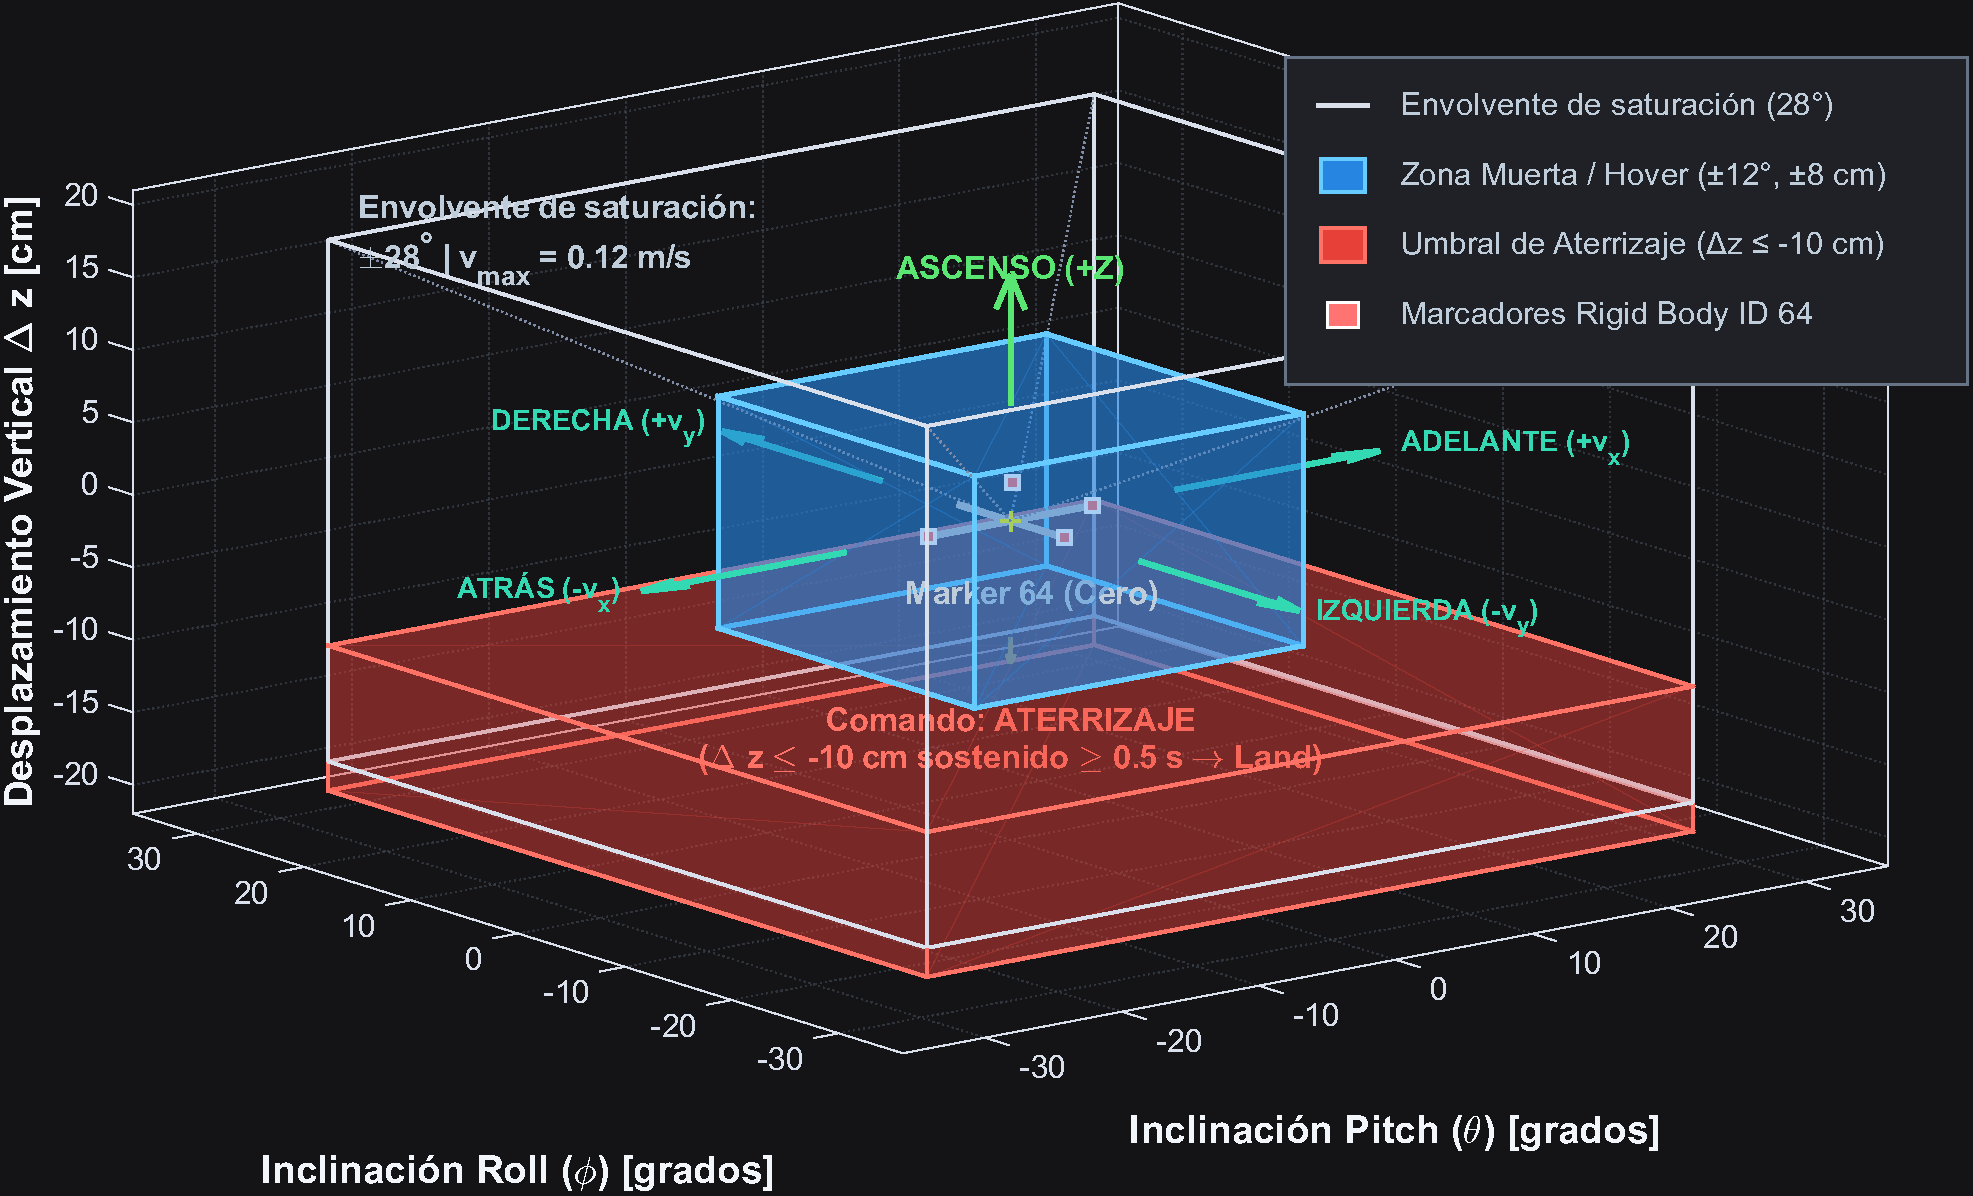
\includegraphics[width=0.78\textwidth]{figuras/joystick_marker_espacio_3d.pdf}%
    }{%
        \fbox{\parbox[c][4cm][c]{0.78\textwidth}{\centering Imagen pendiente: \texttt{figuras/joystick\_marker\_espacio\_3d.pdf}}}%
    }

    \begin{minipage}{0.78\textwidth}
        \footnotesize
        \textit{Nota.} Representación del espacio de control generado mediante el marcador rígido identificado con el número 64. Elaboración propia.
    \end{minipage}
\end{figure}

Para el movimiento vertical se utilizó una zona muerta de $\pm 0.08\ m$. Fuera de esta región, la diferencia de altura se sumaba a una referencia base de $0.50\ m$ sobre el punto de despegue. La altura resultante se limitaba entre $0.25$ y $1.10\ m$.

\section{Pruebas de los controladores}

\subsection{Prueba de control mediante marcador}

La sesión analizada tuvo una duración de $55.69\ s$ y produjo 1072 muestras. La referencia inicial se estableció en $t=0.00\ s$, la solicitud de despegue se registró en $t=2.62\ s$ y la solicitud de aterrizaje se produjo en $t=54.61\ s$. Estos eventos representan el instante en que se solicitaron las acciones, no el momento en que concluyó cada maniobra.

El registro permitió relacionar el movimiento del joystick, las referencias de velocidad y la posición del dron. La Figura~\ref{fig:drive_09} muestra inicialmente un intervalo neutro, seguido de órdenes de subida y combinaciones de movimiento vertical y lateral. Posteriormente se observan desplazamientos hacia la izquierda, adelante y atrás.

Según el resumen de la sesión, la categoría SUBIR acumuló aproximadamente $12.73\ s$, mientras que NEUTRO acumuló $9.14\ s$. Las categorías DERECHA + SUBIR e IZQUIERDA acumularon $8.47\ s$ cada una. Las categorías ATRAS y ADELANTE aparecieron durante $5.51$ y $4.26\ s$, respectivamente.

Estas duraciones se estimaron mediante el número de muestras y el intervalo medio de muestreo. Por ello, deben interpretarse como valores aproximados.

\begin{figure}[htbp]
    \centering
    \caption{Secuencia de comandos durante el control mediante marcador.}
    \label{fig:drive_09}
    \IfFileExists{figuras_drive/figura_09.png}{%
        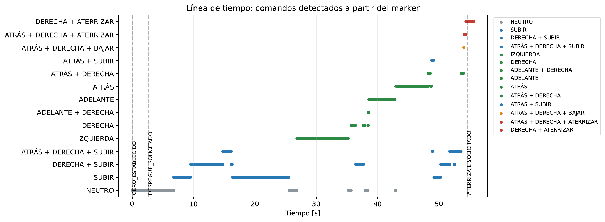
\includegraphics[width=0.78\textwidth]{figuras_drive/figura_09.png}%
    }{%
        \fbox{\parbox[c][4cm][c]{0.78\textwidth}{\centering Imagen pendiente: \texttt{figuras\_drive/figura\_09.png}}}%
    }

    \begin{minipage}{0.78\textwidth}
        \footnotesize
        \textit{Nota.} Cada punto corresponde a una muestra del registro. Las líneas verticales indican el establecimiento de la referencia y las solicitudes de despegue y aterrizaje. Elaboración propia.
    \end{minipage}
\end{figure}

\subsection{Prueba de vuelo mediante el reconocedor gestual integrado}

El reconocedor gestual integró en una misma aplicación la detección de configuraciones de la mano y de movimientos del cuerpo completo. Para comprobar su conexión con el controlador de vuelo se analizaron dos sesiones complementarias con un cuadricóptero Crazyflie y el sistema de posicionamiento del Robotat. La primera utilizó gestos de la mano y la segunda combinó gestos corporales dinámicos con posturas estáticas. Debido a que los registros tuvieron duraciones y condiciones distintas, sus resultados se describen por separado y no constituyen una comparación directa.

\subsubsection*{Prueba con gestos de la mano}

En la sesión basada en gestos de la mano, la duración total fue de aproximadamente 183 s, de los cuales 170 s correspondieron al vuelo. Durante el ensayo se reconocieron y ejecutaron las órdenes de despegue, ascenso, desplazamiento lateral hacia ambos lados, avance, retroceso, seguimiento del marcador y detención. Los desplazamientos producidos por los gestos direccionales fueron de aproximadamente 0.5 a 0.8 m.

La Figura~\ref{fig:drive_10} presenta la cronología de los gestos observados durante la sesión. Las regiones correspondientes a comandos confirmados permiten identificar los intervalos en los que el controlador aceptó cada gesto y lo convirtió en una acción de vuelo. También se muestran los periodos en los que el cuadricóptero permaneció en vuelo, ejecutó una maniobra o mantuvo el seguimiento del marcador. La presencia de intervalos clasificados como \texttt{NO\_GESTURE} indica que el sistema no generó continuamente órdenes de movimiento cuando el operador no mantenía una configuración reconocida.

\begin{figure}[htbp]
    \centering
    \caption{Cronología de los gestos de la mano reconocidos y de los comandos atendidos por el controlador durante la prueba de vuelo.}
    \label{fig:drive_10}
    \IfFileExists{figuras/Timelapse_comandos_drone.pdf}{%
        \includegraphics[width=0.84\textwidth]{figuras/Timelapse_comandos_drone.pdf}%
    }{%
        \fbox{\parbox[c][4cm][c]{0.84\textwidth}{\centering Imagen pendiente: \texttt{figuras/Timelapse\_comandos\_drone.pdf}}}%
    }

    \begin{minipage}{0.84\textwidth}
        \footnotesize
        \textit{Nota.} Elaboración propia.
    \end{minipage}
\end{figure}

La relación entre los gestos detectados, las órdenes enviadas y la posición del cuadricóptero se presenta en la Figura~\ref{fig:drive_11}. Después de confirmarse el gesto de despegue, la altura aumentó desde el nivel del suelo hasta la región de vuelo. Posteriormente, los comandos asociados con el movimiento en los ejes horizontal y vertical produjeron variaciones observables en las coordenadas registradas. Este comportamiento muestra que las detecciones realizadas por la cámara no permanecieron únicamente como resultados de clasificación, sino que fueron traducidas por el controlador en referencias de movimiento para el cuadricóptero.

\begin{figure}[htbp]
    \centering
    \caption{Correspondencia temporal entre los gestos reconocidos, las órdenes enviadas y la posición del cuadricóptero.}
    \label{fig:drive_11}
    \IfFileExists{figuras/07_comandos_y_vuelo.pdf}{%
        \includegraphics[width=0.78\textwidth]{figuras/07_comandos_y_vuelo.pdf}%
    }{%
        \fbox{\parbox[c][4cm][c]{0.78\textwidth}{\centering Imagen pendiente: \texttt{figuras/07\_comandos\_y\_vuelo.pdf}}}%
    }

    \begin{minipage}{0.78\textwidth}
        \footnotesize
        \textit{Nota.} Elaboración propia.
    \end{minipage}
\end{figure}

La trayectoria completa de la prueba se representa en la Figura~\ref{fig:drive_12}. El color de los puntos indica el avance temporal de la sesión y permite observar los desplazamientos efectuados en los tres ejes. El punto de despegue y el final del ensayo se señalan de forma independiente. La trayectoria evidencia que el cuadricóptero respondió a distintas órdenes gestuales y se desplazó dentro del volumen de operación establecido.

\begin{figure}[htbp]
    \centering
    \caption{Trayectoria tridimensional del cuadricóptero durante la prueba de control mediante gestos de la mano.}
    \label{fig:drive_12}
    \IfFileExists{figuras/08_vuelo_3d.pdf}{%
        \includegraphics[width=0.68\textwidth]{figuras/08_vuelo_3d.pdf}%
    }{%
        \fbox{\parbox[c][4cm][c]{0.68\textwidth}{\centering Imagen pendiente: \texttt{figuras/08\_vuelo\_3d.pdf}}}%
    }

    \begin{minipage}{0.68\textwidth}
        \footnotesize
        \textit{Nota.} Elaboración propia.
    \end{minipage}
\end{figure}

La sesión finalizó cuando el mecanismo de seguridad detectó una diferencia de 0.161 m entre la posición estimada por el filtro del cuadricóptero y la posición proporcionada por el sistema de captura de movimiento, valor superior al límite de 0.15 m configurado para la prueba. En ese instante, la tensión de la batería había descendido hasta 2.96 V. Por tanto, la finalización no se atribuyó a una orden gestual incorrecta, sino a la activación de una condición de seguridad del sistema de vuelo. En conjunto, el ensayo permitió comprobar empíricamente la cadena completa de operación: adquisición de la imagen, reconocimiento del gesto, confirmación temporal, generación del comando y desplazamiento físico del cuadricóptero.

\subsubsection*{Prueba con gestos corporales}

En la sesión de gestos corporales se observó la alternancia entre los comandos dinámicos y las posturas estáticas de navegación. La Figura~\ref{fig:drive_13} presenta un registro de aproximadamente 73 s y 2120 cuadros procesados, con los gestos detectados, su confirmación y los estados de vuelo informados por el controlador.

La secuencia comenzó con señalero asociado a una solicitud de despegue. A continuación, aplaudir cambió el sistema al modo estático, en el que se registraron intervalos de navegación hacia la derecha, la izquierda y adelante, además de detecciones de ascenso y descenso. Más adelante, otro aplauso restableció el modo dinámico y señalero generó una solicitud de aterrizaje; al final del registro aparece una nueva solicitud de despegue.

\begin{figure}[htbp]
    \centering
    \caption{Secuencia de comandos corporales y cambios de modo durante una prueba del controlador.}
    \label{fig:drive_13}
    \IfFileExists{figuras/comandos_cuerpo_completo.pdf}{%
        \includegraphics[width=0.78\textwidth]{figuras/comandos_cuerpo_completo.pdf}%
    }{%
        \fbox{\parbox[c][4cm][c]{0.78\textwidth}{\centering Imagen pendiente: \texttt{figuras/comandos\_cuerpo\_completo.pdf}}}%
    }

    \begin{minipage}{0.78\textwidth}
        \footnotesize
        \textit{Nota.} Las franjas de fondo representan los estados de vuelo y maniobra; las marcas distinguen los gestos confirmados de las detecciones sin confirmar. Las líneas verticales señalan las acciones asociadas a señalero y aplaudir. Elaboración propia.
    \end{minipage}
\end{figure}

El registro permite relacionar las detecciones corporales con las decisiones del controlador, pero no mide por sí solo la exactitud del reconocedor ni el desplazamiento alcanzado por el dron. Los intervalos \texttt{NO\_GESTURE} indican ausencia de un gesto reconocido, no necesariamente una detención del vuelo. Asimismo, las líneas de despegue y aterrizaje representan solicitudes de acción, no la confirmación de que cada maniobra haya concluido.

En conjunto, ambas sesiones permitieron comprobar el funcionamiento de las entradas de mano y cuerpo del reconocedor integrado y su conexión con el controlador de un único cuadricóptero. Debido a que se realizaron en condiciones diferentes, estos registros se emplean como pruebas de integración y no como una evaluación comparativa de exactitud.

\chapter{Reconocimiento de gestos dinámicos}

El sistema de reconocimiento de gestos dinámicos se desarrolló para incorporar comandos definidos mediante movimientos corporales. A diferencia de los gestos estáticos de navegación, estos comandos se caracterizaron por la trayectoria descrita por las articulaciones durante un intervalo. Por esta razón, su reconocimiento requirió registrar una secuencia de poses, identificar el inicio y el final del movimiento y comparar la trayectoria obtenida con muestras previamente almacenadas.

Para realizar esta comparación se implementó un reconocedor basado en alineamiento temporal dinámico, conocido como Dynamic Time Warping (DTW). El método permitió comparar ejecuciones con diferencias en su ritmo. El reconocedor se integró con el sistema de estimación de pose corporal y con el controlador de vuelo, de manera que los gestos aceptados pudieran convertirse en acciones para el cuadricóptero.

\section{Definición del vocabulario dinámico}

El vocabulario dinámico se definió a partir de acciones que requerían activar eventos o comportamientos de vuelo. Se seleccionaron cinco gestos: \textit{señalero}, \textit{aplaudir}, \textit{ven acá}, \textit{arco} y \textit{círculo}. La Tabla~\ref{tab:drive_01} presenta la acción asignada a cada uno.

\begin{table}[htbp]
    \centering
    \caption{Gestos dinámicos y acciones asociadas.}
    \label{tab:drive_01}
    \begin{tabularx}{0.92\textwidth}{@{}lX@{}}
        \toprule
        Gesto & Acción asociada \\
        \midrule
        Señalero & Despegar o aterrizar \\
        Aplaudir & Cambiar entre los modos dinámico y estático \\
        Ven acá & Activar el seguimiento del marcador del operador \\
        Círculo & Activar la órbita alrededor del marcador \\
        Arco & Solicitar una pirueta \\
        \bottomrule
    \end{tabularx}

    \begin{minipage}{0.92\textwidth}
        \footnotesize
        \textit{Nota.} Acciones asignadas en la integración del vocabulario con el controlador de vuelo. Elaboración propia.
    \end{minipage}
\end{table}

La Figura~\ref{fig:drive_14} muestra las trayectorias de las muñecas durante los cinco gestos. La línea azul representa el recorrido de la muñeca derecha y la línea magenta el de la izquierda. Los círculos indican el inicio de cada trayectoria y las puntas señalan su final. También se muestran las configuraciones inicial y final del esqueleto, observadas de frente y de perfil.

\begin{figure}[htbp]
    \centering
    \caption{Trayectorias de las muñecas para los gestos dinámicos que conforman el vocabulario.}
    \label{fig:drive_14}
    \IfFileExists{figuras/gestos_dinamicos.pdf}{%
        \includegraphics[width=0.72\textwidth]{figuras/gestos_dinamicos.pdf}%
    }{%
        \fbox{\parbox[c][4cm][c]{0.72\textwidth}{\centering Imagen pendiente: \texttt{figuras/gestos\_dinamicos.pdf}}}%
    }

    \begin{minipage}{0.72\textwidth}
        \footnotesize
        \textit{Nota.} Representación de las trayectorias y configuraciones corporales. Elaboración propia.
    \end{minipage}
\end{figure}

\section{Registro de las muestras}

Para construir el conjunto de datos se grabaron distintas repeticiones de cada gesto. Las secuencias incluyeron los puntos articulares proporcionados por el estimador de pose y sus instantes de captura. Cada ejecución se identificó mediante la etiqueta del gesto y el participante correspondiente. También se registraron movimientos ajenos al vocabulario bajo la etiqueta \textit{otro}, destinados a construir y evaluar el mecanismo de rechazo.

La recolección reunió 690 muestras de 13 participantes, con variaciones en la orientación respecto de la cámara y en la ejecución de los gestos. Cada muestra correspondió a una ejecución completa, no a un cuadro individual. La captura se realizó en dos grupos: cinco participantes aportaron 263 secuencias —222 del vocabulario y 41 de movimientos ajenos—, y ocho participantes adicionales aportaron 427. Durante la validación, las muestras de una misma persona se mantuvieron en una sola partición. Los informes disponibles evaluaron los grupos por separado; la matriz de confusión y la comparación de umbrales presentadas corresponden al primero.

Se denominó muestra a cada ejecución completa registrada, con su etiqueta y participante; una plantilla fue la representación preprocesada de una muestra utilizada como referencia de comparación. Por tanto, no se trató de dos tipos distintos de grabación: una muestra podía convertirse en plantilla o reservarse para prueba según la partición de validación. Las plantillas conservaron la clase y las trayectorias normalizadas de muñecas y codos; el banco almacenó, además, los parámetros de procesamiento y los umbrales de aceptación.

\section{Preprocesamiento y clasificación mediante DTW}

Antes de aplicar DTW, las poses se transformaron al sistema de referencia corporal y se normalizaron mediante la escala del torso. Estas operaciones buscaron reducir la influencia de la posición del participante, su orientación y sus dimensiones corporales sobre las distancias utilizadas para clasificar los gestos. Para representar cada instante se utilizaron las coordenadas tridimensionales de la muñeca derecha, la muñeca izquierda, el codo derecho y el codo izquierdo.

Los cuadros en los que alguna de las articulaciones requeridas no estaba disponible se marcaron como datos no válidos. Para procesar una secuencia se exigió una cobertura mínima del 70 \% de poses utilizables y al menos cuatro cuadros válidos. Esta condición limitó la clasificación de movimientos con información incompleta.

Se implementó una segmentación basada en el movimiento de las muñecas. Esta decisión respondió a las diferencias de duración entre los gestos, puesto que una ventana temporal fija podía cortar una ejecución larga o incorporar períodos excesivos de reposo en una corta. La rapidez conjunta de las muñecas se calculó a partir del cambio de sus posiciones entre cuadros consecutivos y del tiempo transcurrido. Para reducir el efecto de variaciones aisladas del estimador de pose, la señal se suavizó mediante un promedio móvil de tres valores válidos de rapidez.

Los cuadros sin una pose utilizable se trataron como datos ausentes, no como periodos de quietud, para evitar que una pérdida temporal de detección cerrara prematuramente el segmento. Se rechazaron las secuencias cuya duración, después del recorte, quedaba fuera del intervalo de 1 a 7 s. Tras cada cierre se estableció una espera de 1 s antes de admitir otro segmento, con el fin de reducir las activaciones producidas por los movimientos de transición. El reconocimiento se produjo al finalizar cada segmento. Por tanto, el tiempo de respuesta incluyó la duración del movimiento y la espera necesaria para confirmar su cierre.

Cuando finalizaba un segmento, su trayectoria se comparaba con todas las plantillas de gestos almacenados. La distancia local se calculó mediante la norma euclidiana de los vectores de características. Para limitar la deformación temporal se utilizó una banda de Sakoe–Chiba parametrizada con una fracción de 0.25 de la longitud de las secuencias.

El costo acumulado se dividió entre el número de pasos del camino de alineamiento obtenido. Para cada clase se conservó la menor distancia entre el segmento observado y las plantillas pertenecientes a esa clase.

Se seleccionó como candidato el gesto cuya plantilla produjo la menor distancia normalizada respecto del segmento observado.

La selección del candidato no fue suficiente para emitir un comando. El segmento se rechazó cuando la distancia superó el umbral de aceptación o cuando la plantilla más cercana perteneció a la clase \textit{otro}. Los segmentos aceptados se enviaron a la máquina de modos, que determinó si la acción estaba permitida en el estado actual.

En la configuración construida con 263 muestras de cinco participantes se obtuvieron los umbrales presentados en la Tabla~\ref{tab:drive_02}. Estos valores corresponden al banco construido con ese conjunto completo; durante la validación anidada se calcularon umbrales independientes en cada partición.

\begin{table}[htbp]
    \centering
    \caption{Umbrales por gesto del banco construido con 263 muestras.}
    \label{tab:drive_02}
    \begin{tabularx}{0.92\textwidth}{@{}lX@{}}
        \toprule
        Gesto & Umbral DTW \\
        \midrule
        Aplaudir & 0.373 \\
        Ven acá & 0.475 \\
        Círculo & 0.511 \\
        Señalero & 0.701 \\
        Arco & 0.716 \\
        \bottomrule
    \end{tabularx}

    \begin{minipage}{0.92\textwidth}
        \footnotesize
        \textit{Nota.} Umbrales calculados a partir de las distancias entre secuencias normalizadas por la escala corporal. Elaboración propia.
    \end{minipage}
\end{table}

El uso de umbrales independientes permitió ajustar la aceptación de cada clase a la distribución de sus distancias de acierto y de error. En esta configuración, \textit{aplaudir} recibió un umbral más estricto que \textit{arco}. Estas diferencias reflejaron el comportamiento observado en las muestras utilizadas para construir el banco.

El reconocedor también calculó la diferencia entre la distancia del mejor candidato y la del segundo mejor candidato. Sin embargo, el margen mínimo se configuró en cero, por lo que este valor no impuso una separación positiva adicional entre clases. El rechazo dependió del umbral de distancia y de la selección de la clase \textit{otro}.

\section{Evaluación del reconocedor}

La evaluación del reconocedor se realizó sobre las secuencias grabadas mediante validación cruzada dejando fuera a un participante, denominada Leave-One-Subject-Out (LOSO). En cada iteración se reservaron todas las muestras de una persona como casos de prueba; las secuencias preprocesadas de las demás personas formaron el banco de plantillas de referencia. Así, ninguna ejecución de la persona evaluada se utilizó como plantilla para reconocerla.

La selección de los umbrales se efectuó mediante una validación anidada dentro de los participantes disponibles para entrenamiento. De esta manera, las muestras del participante evaluado no intervinieron en la selección de los límites de aceptación. El procedimiento se repitió hasta evaluar a todos los participantes.

Se calcularon la exactitud global y las métricas por clase. La exactitud expresó la proporción de muestras clasificadas correctamente, incluidos los rechazos correctos. La precisión indicó cuántas de las predicciones asignadas a una clase eran correctas; la exhaustividad, cuántas muestras reales de esa clase se reconocieron. La puntuación F1 combinó precisión y exhaustividad mediante su media armónica, de modo que un valor alto requería un buen desempeño en ambas. Se empleó macro-F1 para promediar, con igual peso, las puntuaciones de los cinco gestos y de la categoría de rechazo, sin favorecer a las clases con más muestras.

La evaluación se efectuó sobre secuencias grabadas y preprocesadas. Por tanto, sus resultados caracterizaron la clasificación y el rechazo de esas secuencias, pero no constituyeron por sí solos una medición de los falsos comandos por minuto durante el uso continuo del sistema.

En el conjunto de 263 muestras de cinco participantes, la clasificación por vecino más cercano sin aplicar umbrales de aceptación obtuvo una exactitud de 79.5 \%. Al incorporar el rechazo y seleccionar los umbrales por clase mediante validación LOSO anidada, la exactitud fue de 77.6 \% y el macro-F1 fue de 0.782. La primera configuración asignaba la clase de la plantilla más cercana; la segunda también permitía descartar segmentos según los umbrales calculados sin utilizar al participante evaluado.

La Figura~\ref{fig:drive_15} presenta los resultados de la configuración con umbrales por clase. Las filas corresponden a la clase real y las columnas a la salida del reconocedor. La categoría \textit{Movimiento ajeno} identifica las muestras externas al vocabulario, mientras que \textit{Sin comando} representa la decisión de rechazo.

\begin{figure}[htbp]
    \centering
    \caption{Matriz de confusión del reconocedor de gestos dinámicos mediante DTW.}
    \label{fig:drive_15}
    \IfFileExists{figuras/matriz_confusion_dtw.pdf}{%
        \includegraphics[width=0.72\textwidth]{figuras/matriz_confusion_dtw.pdf}%
    }{%
        \fbox{\parbox[c][4cm][c]{0.72\textwidth}{\centering Imagen pendiente: \texttt{figuras/matriz\_confusion\_dtw.pdf}}}%
    }

    \begin{minipage}{0.72\textwidth}
        \footnotesize
        \textit{Nota.} Validación LOSO anidada con umbrales por clase sobre 263 muestras de cinco participantes. Porcentajes normalizados por fila y conteos entre paréntesis. Elaboración propia.
    \end{minipage}
\end{figure}

Señalero obtuvo la mayor exhaustividad, con 93.2 \%, seguido de círculo, con 84.8 \%. Aplaudir y ven acá alcanzaron 77.8 \% y 77.3 \%, respectivamente. Arco presentó el menor valor, con 55.8 \%; su principal dificultad fue el rechazo de 17 de sus 43 muestras. Asimismo, el sistema rechazó correctamente 31 de los 41 movimientos ajenos al vocabulario, equivalentes al 75.6 \%.

Al comparar las dos estrategias de selección de umbrales mediante validación anidada, ambas obtuvieron una exactitud de 77.6 \%. El macro-F1 pasó de 0.771 con un umbral único a 0.782 con umbrales por clase. La cantidad de movimientos ajenos aceptados como comandos se redujo de 17 a 10 entre 41 muestras. A su vez, los gestos válidos rechazados aumentaron de 18 a 37 entre 222 muestras.

Esta comparación mostró un compromiso entre rechazar movimientos ajenos y aceptar variaciones legítimas de los gestos. Los umbrales por clase redujeron las aceptaciones incorrectas, pero incrementaron los falsos rechazos. Superar el umbral tampoco garantizó una clasificación correcta, pues un gesto válido podía confundirse con otra clase.

En otra configuración se añadieron muestras de \textit{saludar} y \textit{reposo} al conjunto de rechazo. La exactitud obtenida fue de 69.5 \%. El análisis señaló confusiones entre \textit{saludar} y \textit{ven acá}, lo que mostró que ampliar el conjunto de movimientos ajenos no mejoraba necesariamente la separación entre clases.

En el grupo de ocho participantes, con 427 muestras, la validación anidada con umbrales por clase obtuvo una exactitud de 77.1 \% y un macro-F1 de 0.774. Estos resultados y los del grupo de cinco participantes pertenecen al mismo proceso de recolección de 13 personas, pero se calcularon por separado. Por ello, la matriz de la Figura~\ref{fig:drive_15} y sus porcentajes no representan una validación conjunta de las 690 muestras.

Finalmente, la validación por participante permitió evaluar la generalización entre las personas registradas, pero el tamaño de los conjuntos limitó el alcance de los resultados. Las cifras obtenidas describieron el comportamiento sobre las muestras disponibles y no demostraron un desempeño equivalente para cualquier operador o condición de captura.

\section{Integración con el controlador de vuelo}

El reconocedor se conectó al controlador mediante una máquina de estados con dos modos: dinámico y estático. El gesto aplaudir permitía alternar entre ambos sin solicitar el aterrizaje y cancelaba el comportamiento activo para solicitar vuelo estacionario. En modo dinámico se admitían señalero, ven acá, círculo y arco; en modo estático se habilitaban las posturas de navegación y se mantenía activo el reconocimiento de aplaudir para cambiar de modo.

La máquina de estados consultaba al controlador si el dron estaba en el aire antes de autorizar una acción. Señalero solicitaba despegar o aterrizar según ese estado, mientras que los comportamientos de seguimiento, órbita y pirueta solo se admitían en vuelo. La traducción de cada decisión a las órdenes de vuelo correspondía al controlador, no al clasificador DTW.

El paro estático tenía prioridad sobre ambos modos. La postura de brazos cruzados en X sobre la cabeza solicitaba frenar al mantenerse durante 0.35 s, aterrizar al alcanzar 1 s y cortar los motores al sostenerse durante 3 s. Mientras permanecía activa, se bloqueaban los demás comandos gestuales. Esta separación evitaba interpretar las posturas intermedias de un movimiento dinámico como órdenes estáticas de navegación.
